% \iffalse
\let\negmedspace\undefined
\let\negthickspace\undefined
\documentclass[beamer]{IEEEtran}
\usepackage{cite}
\usepackage{amsmath,amssymb,amsfonts,amsthm}
\usepackage{algorithmic}
\usepackage{graphicx}
\usepackage{textcomp}
\usepackage{xcolor}
\usepackage{txfonts}
\usepackage{listings}
\usepackage{enumitem}
\usepackage{mathtools}
\usepackage{gensymb}
\usepackage{comment}
\usepackage[breaklinks=true]{hyperref}
\usepackage{tkz-euclide} 
\usepackage{listings}
\usepackage{gvv}                                        
\def\inputGnumericTable{}                                 
\usepackage[latin1]{inputenc}                                
\usepackage{color}                                            
\usepackage{array}                                            
\usepackage{longtable}                                       
\usepackage{calc}                                             
\usepackage{multirow}                                         
\usepackage{hhline}                                           
\usepackage{ifthen}                                           
\usepackage{lscape}
\usepackage[export]{adjustbox}

\newtheorem{theorem}{Theorem}[section]
\newtheorem{problem}{Problem}
\newtheorem{proposition}{Proposition}[section]
\newtheorem{lemma}{Lemma}[section]
\newtheorem{corollary}[theorem]{Corollary}
\newtheorem{example}{Example}[section]
\newtheorem{definition}[problem]{Definition}
\newcommand{\BEQA}{\begin{eqnarray}}
\newcommand{\EEQA}{\end{eqnarray}}
\newcommand{\define}{\stackrel{\triangle}{=}}
\theoremstyle{remark}
\newtheorem{rem}{Remark}
\begin{document}
\parindent 0px
\bibliographystyle{IEEEtran}

\title{Gate EE - 18}
\author{EE23BTECH11216 - P.kalyan$^{}$% <-this % stops a space
}
\maketitle
\newpage
\bigskip

\renewcommand{\thefigure}{\theenumi}
\renewcommand{\thetable}{\theenumi}
\section*{Question}
The Fourier transform x$\brak{\omega}$ of  the signal x\brak{t} is given by

\[
X(\omega) = 
\begin{cases} 
1, \text{for } |\omega| < \omega_0 \\
0, \text{for } |\omega| > \omega_0 
\end{cases}
\]

\text{(A) } x\brak{t} \text{ tends to be an impulse as } $W_0$ $\rightarrow \infty$.

\text{(B) } x\brak{0} \text{ decreases as } $W_0$ \text{ increases.}

\text{(C) At } t = $\frac{\pi}{2W_0}$, \quad x\brak{t} = -$\frac{1}{\pi}$.

\text{(D) At } t = $\frac{\pi}{2W_0}$, \quad x\brak{t} = $\frac{1}{\pi}$. \hfill\brak{\text{GATE EE 2023}}


 \section*{solution}


\begin{center}
    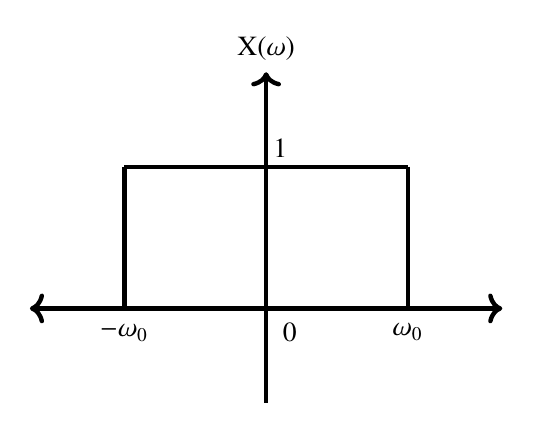
\begin{tikzpicture}[scale=0.6, ultra thick]
        \draw[->] (0,-2) -- (0,5);
        \draw (0,5.5) node {X($\omega$)};
        \draw (0.5,-0.5)  node{0};
        \draw[<->]  (-5,0) -- (5,0);
        \draw  (3,3) -- (3,0);
        \draw (0.3,3.4) node{1};
        \draw (-3,3) -- (3,3);
        \draw (-3,3)--(-3,0);
        \draw (-3,-0.5) node {$-\omega_0$};
        \draw (3,-0.5) node {$\omega_0$};
    \end{tikzpicture}
\end{center}

By taking inverse Fourier transform,
\begin{align}
x\brak{t} = \frac{\sin\brak{\omega_0 t}}{\pi t}
\end{align}

\begin{align}
& x\left(\frac{\pi}{2 \omega_0}\right) =\frac{2 \omega_0}{\pi^2}
\end{align}

So, option \brak{C} and \brak{D} are wrong.

\begin{align}
x\brak{0}=\lim_{t\to 0}\frac{\sin \omega_0 t}{\pi t}=\frac{\omega_0}{\pi}
\end{align}

So, $x\brak{0} \propto \omega_0 \Rightarrow$ Option \brak{B} is wrong.\\

When $\omega \rightarrow \infty$, $X\brak{\omega}$ will be a D.C signal and inverse Fourier transform of a D.C signal will be impulse signal\\[3ex]
So, option \brak{A} is correct


\end{document}
